\section{Mechanistic accounting of margin drift}

The broad panel shows staged answer formation. The instrumented panel asks what can be said about the motion itself. For each layer, the cache contains margin drift along with attention and MLP scalar contributions. A linear drift decomposition reaches held-out $R^2$ between \MechanisticMinHeldoutRtwo{} and \MechanisticMaxHeldoutRtwo{} across the three instrumented models, which is strong enough to treat the decomposition as useful accounting of readout motion.

\begin{figure}[tbp]
\centering
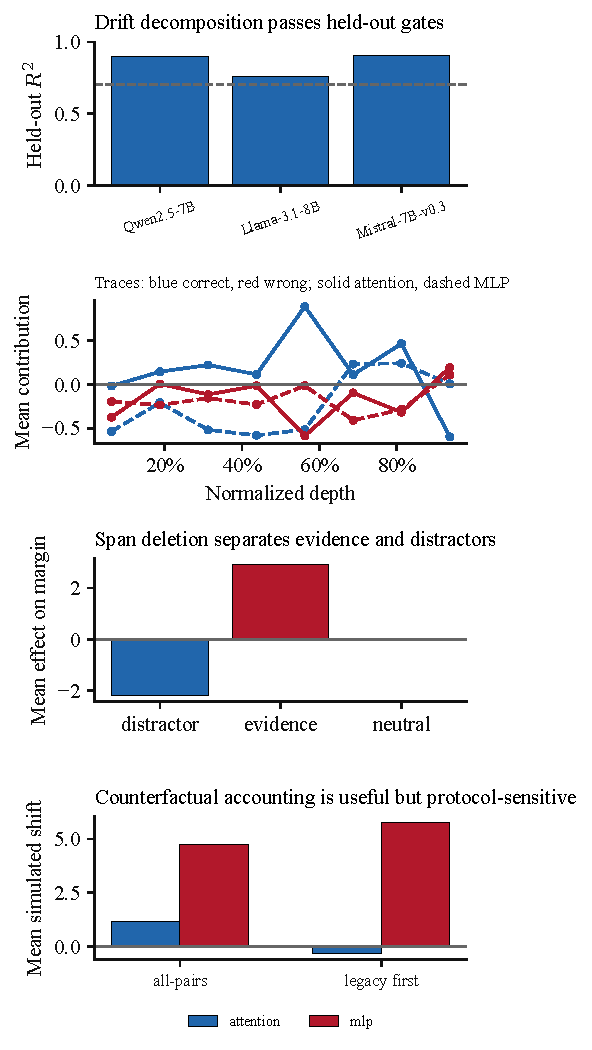
\includegraphics[width=\linewidth]{figure5_mechanistic_accounting.pdf}
\caption{\textbf{Mechanistic accounting in the instrumented panel.} Attention/MLP scalars reconstruct margin drift with held-out fits; component traces differ by trajectory type; span deletion separates evidence from distractors; and substitution accounting is informative but protocol-sensitive.}
\label{fig:mechanistic}
\end{figure}

The panels in Figure~\ref{fig:mechanistic} play different roles. The held-out fits show that a low-dimensional accounting model captures margin drift; the trace panel shows that component contributions vary by trajectory type; span deletion is the strongest input-level intervention; and substitution is useful but more protocol-sensitive.

The strongest intervention evidence is span deletion. Evidence spans have positive mean effects on the decision margin, while distractor spans have negative mean effects; the mean evidence-minus-distractor gap is \SpanEvidenceDistractorGap{} logit-margin units. The effect remains significant under Benjamini--Hochberg correction, and observed effects exceed shuffled and sign-flipped controls.

\begin{table}[tbp]
\centering
\small
\begin{tabularx}{\linewidth}{@{}lX@{}}
\toprule
\textbf{Mechanistic artifact} & \textbf{Value} \\
\midrule
Instrumented models & 3 \\
Component-depth summary rows & 288 \\
Minimum held-out drift R-squared & 0.76 \\
Mean evidence-minus-distractor gap & 5.10 \\
All-pairs MLP substitution mean shift & 4.74 \\
All-pairs attention substitution mean shift & 1.18 \\
\bottomrule
\end{tabularx}

\caption{\textbf{Mechanistic artifact summary.} All values are regenerated from the released mechanistic table.}
\label{tab:mechanistic-summary}
\end{table}

Cached counterfactual accounting adds a second, more conditional result. Under order-invariant all-pairs substitution, attention shifts failing trajectories by \SubstitutionAttentionMean{} logits on average, while MLP shifts them by \SubstitutionMLPMean{} logits on average. This supports the qualitative conclusion that MLP contributions are often more transferable in the cached accounting setup. It is not an unconditional circuit claim: the exact sign and magnitude vary with pairing protocol, layer range, and normalization.
